\documentclass{article}
\usepackage{amsmath,amsthm,amssymb,amsfonts}
\usepackage{setspace,enumitem}
\usepackage{graphicx}
\usepackage{hyperref}
\usepackage{natbib}
\usepackage{afterpage}
\usepackage{xcolor}
\usepackage{etoolbox}
\usepackage{booktabs}
\usepackage{pdfpages}
\usepackage{multicol}
\usepackage{geometry}
\usepackage{accents}
\usepackage{bbm}
\usepackage{placeins}
\hypersetup{
	colorlinks,
	linkcolor={blue!90!black},
	citecolor={red!90!black},
	urlcolor={blue!90!black}
}

\newtheorem{theorem}{Theorem}
\newtheorem{assumption}{Assumption}
\newtheorem{definition}{Definition}
\newtheorem{lemma}{Lemma}
\setlength{\parindent}{0cm}
\geometry{margin = 1in}

\newcommand{\R}{\mathbb{R}}
\newcommand{\ubar}[1]{\underaccent{\bar}{#1}}
\newcommand{\Int}{\text{Int}}
\newcommand{\xbf}{\mathbf{x}}
\newcommand{\Abf}{\mathbf{A}}
\newcommand{\Bbf}{\mathbf{B}}
\newcommand{\Gbf}{\mathbf{G}}
\newcommand{\bbf}{\mathbf{b}}
\newcommand{\one}{\mathbbm{1}}

\newtoggle{extended}
\settoggle{extended}{false}

\title{ECON 810: Homework 2}
\author{Alex von Hafften }

\begin{document}

\maketitle

\begin{itemize}

\section{Part 1: Data}

\subsection{Earnings gains while employed}

\item I used PSID data with the following filters:

\begin{itemize}

\item Main sample. No SEO oversample.

\item Years 1978-1997 inclusive.

\item Ages 25 to 60 inclusive.

\item Annual hours worked \texttt{e11101} of at least 1800 (= 52 weeks per year minus two weeks for vacation times 36 hours).

\item I use variable \texttt{i11103} (description ``HH Labor Income") as my income variable, $Y_{it}$. I drop observations with zero income and over $e^{12} \approx 163000$.

\item I limit the growth in earnings to doubling or less (i.e. a hundred percent increase in earnings).

\end{itemize} 

\item I compute an annual change in earnings of 7.35\%.

\item See \texttt{part\_1\_1.R} for implementation.

\subsection{Earnings losses while unemployed}

\item I use the iid normal shocks to individuals income over time $\varepsilon \sim_{iid} N(0, 1000)$.

\item See \texttt{part\_1\_2.jl} for the implementation.

\item $\beta_k \approx 0$ for $k \in \{-4,..., -1\}$ and $\beta_k \approx -9000$ for $k \in \{0,..., 5\}$.  This makes sense because the income shock from job loss is permanent.

\item $\gamma_t$ start at around -5000 and increase by 1000 each period. This makes sense because it captures the incremental increase in income.

\begin{tabular}{lr}
\toprule
          & \multicolumn{1}{c}{earnings} \\ 
\cmidrule(lr){2-2} 
          &                          (1) \\ 
\midrule
dm4       &                      113.728 \\ 
          &                     (87.470) \\ 
dm3       &                      122.149 \\ 
          &                     (87.470) \\ 
dm2       &                        7.981 \\ 
          &                     (87.470) \\ 
dm1       &                       80.500 \\ 
          &                     (87.470) \\ 
d0        &                 -8842.457*** \\ 
          &                     (87.470) \\ 
dp1       &                 -8895.236*** \\ 
          &                     (87.470) \\ 
dp2       &                 -8969.840*** \\ 
          &                     (87.470) \\ 
dp3       &                 -8885.697*** \\ 
          &                     (87.470) \\ 
dp4       &                 -8891.502*** \\ 
          &                     (87.470) \\ 
dp5       &                 -8935.596*** \\ 
          &                     (87.470) \\ 
\midrule
\midrule
Estimator &                          OLS \\ 
\midrule
$N$       &                       11,000 \\ 
$R^2$     &                        0.941 \\ 
\bottomrule
\end{tabular}


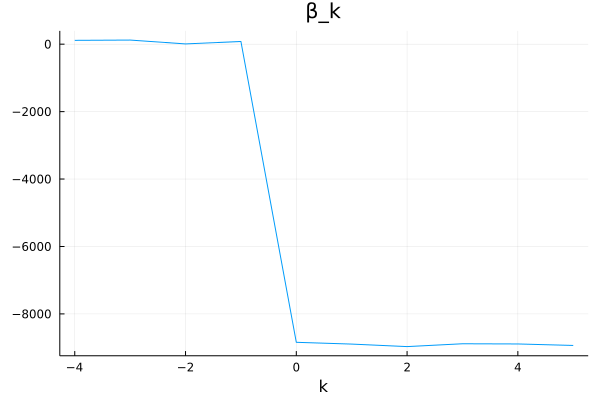
\includegraphics[scale=0.5]{part_1_2_beta}

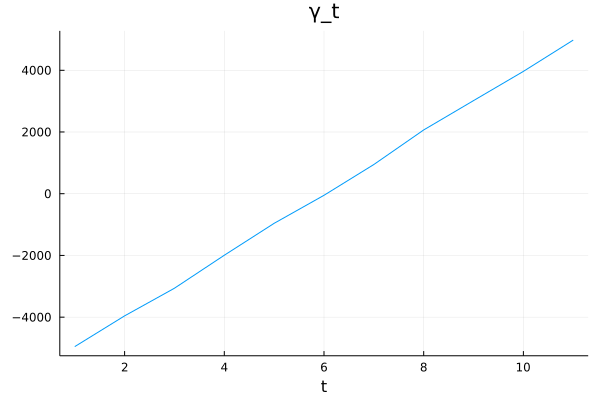
\includegraphics[scale=0.5]{part_1_2_gamma}

\pagebreak

\section{Part 2: Model}

\item I use $\psi_e = 0.5$ and $\psi_u = 0.2$.

\item I use $b = 0.5$.

\item The search effort policy function ends up equaling one for all levels and human capital period expect for the end.  Below is the search policy function for the every three months in the last two years.  As an unemployed worker get closer to the end of the model, they spend less effort searching for more levels of human capital.

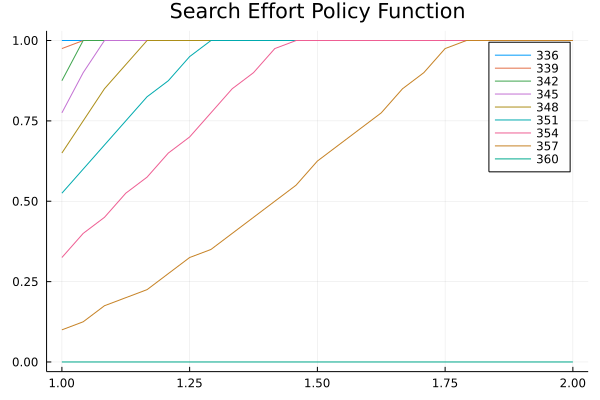
\includegraphics[scale=0.5]{search_pf}

\item Below is the reservation wage policy function for every five years starting at 2.5 years.  It is generally increasing in human capital.

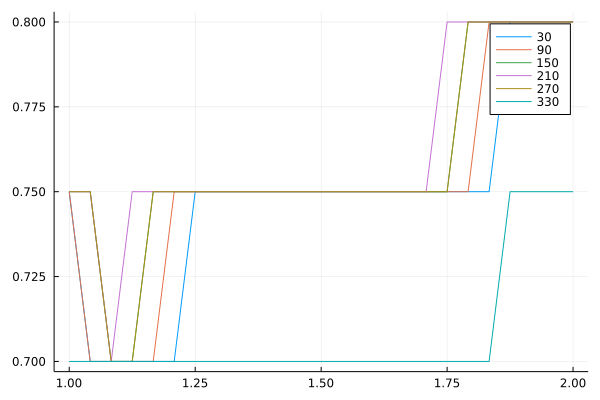
\includegraphics[scale = 0.5]{reservation_wage_pf}

\pagebreak

\item I simulated a panel of 10000 individuals.  Below is the mean level of human capital by employment status.  The initial spike of high human capital in the unemployed and low human capital in the employed makes sense because everyone starts off as unemployed.  I'm surprised by how constant the mean level is over time.  Nearing death, the human capital level of employed starts to dip and the unemployed starts to rise.

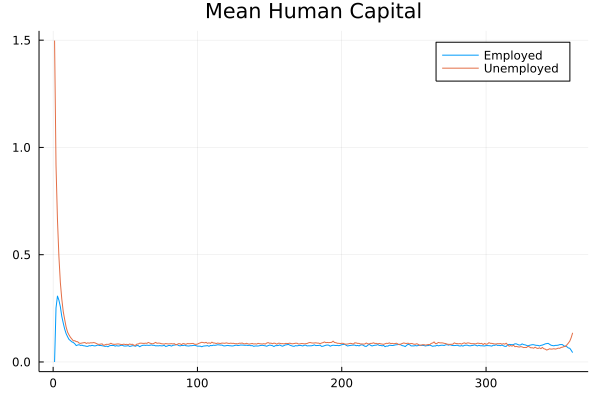
\includegraphics[scale=0.5]{mean_human_capital}

\item I compute an average earnings growth when employed of 32.16 percent, which is substantially larger than the value I computed from the data.

\item I searched through the simulations for job losses and below plot the average earnings from six months before to 2 years after job loss. We see a similar pattern to Davis and von Wachter (2011) with a drop in earnings and then a slow recovery but never reaching the same level.

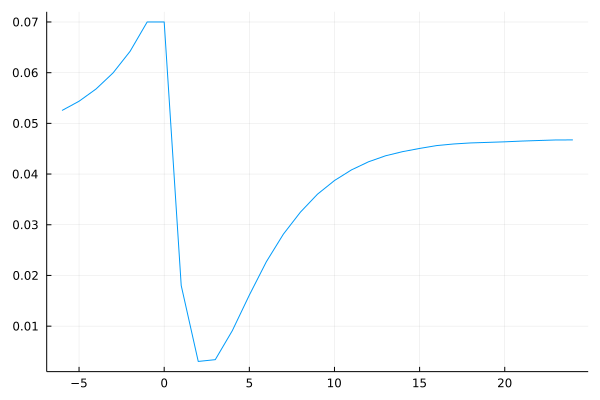
\includegraphics[scale=0.5]{jl}

\item See \texttt{part\_2\_XXX.jl} files for implementation.

\begin{itemize}
\item See \texttt{part\_2\_model.jl} contains code to estimate the model.
\item See \texttt{part\_2\_simulation.jl} contains code to simulate the model.
\item See \texttt{part\_2\_run.jl} contains runs the estimate and simulation and creates charts.
\end{itemize}
\end{itemize}
\end{document}

